\documentclass[a4paper, 11pt]{article}

\usepackage[ngerman, english]{babel}
\usepackage[latin9]{inputenc}
\usepackage{color}
\usepackage{graphicx}
\usepackage{multirow}
\usepackage[verbose]{hyperref}
\usepackage[verbose]{placeins}
\usepackage{amsmath,mathtools}
\usepackage{amssymb}
\usepackage{bm}
\usepackage{url}
\usepackage{subfig}
\usepackage{wasysym}
\usepackage{fancyhdr}
\usepackage[top=1.0in, bottom=0.9in, left=0.8in, right=0.8in]{geometry}
\usepackage{datetime}
\usepackage{verbatim}
\usepackage{siunitx}
\usepackage{fancybox}
\usepackage{empheq}
\usepackage{braket}
\usepackage{multicol}
\usepackage{listings}

\usepackage[edges]{forest}
\usepackage{calc}

\usepackage[]{algorithm2e}

\forestset{
  declare toks={my label}{},
  declare toks={my details}{},
  declare boolean={my icon}{0},
  minecraft schematic/.style={
    for tree={
      folder,
      font=\sffamily,
      grow'=0,
      text width=155mm,
    },
    before typesetting nodes={
      for tree={
        split option={content}{:}{my label,my details},
        delay={
          content/.process={On=?_OOw3}{my icon}{1}{\makebox[\iconwidth+\iconmargin]{}}{}{my label}{my details}{##1\textbf{##2:} ##3},
        },
      },
    },
  },
  icon/.style={
    my icon,
    tikz+={
      \pic at ([xshift=\iconmargin,yshift=-.1*\baselineskip].north west) {my file={#1}};
    },
    edge path'/.expanded={
      ([xshift=\forestregister{folder indent}]!u.parent anchor) |- ([xshift=-.5*\iconmargin,yshift=-.5*\iconheight].north west)
    },
  }
}
\tikzset{
  my file/.pic={
    \draw [icon/.cd, style, #1] (0,-\iconheight) |- +([xshift=-.2*\iconwidth]\iconwidth,\iconheight) edge +([yshift=-.2*\iconwidth]\iconwidth,\iconheight) |- +([yshift=-.2*\iconwidth]\iconwidth,\iconheight) |- cycle;
  },
  icon/.search also={/tikz},
  icon/.cd,
  width/.store in=\iconwidth,
  height/.store in=\iconheight,
  margin/.store in=\iconmargin,
  style/.style={fill=gray!50!blue!25},
  width=7.5pt,
  height=10pt,
  margin=2.5pt,
  main/.style={inner color=white, outer color=red},
  file/.style={inner color=white, outer color=white},
  dim/.style={fill=gray!25},
  elk/.style={top color=blue, bottom color=blue, middle color=cyan},
}


% literature
\usepackage[style=phys,maxbibnames=6,articletitle=true,biblabel=brackets,%
  chaptertitle=true,pageranges=true,eprint=true, natbib=true, block=space, backend=bibtex, sorting=none]{biblatex}

\bibliography{db}
\defbibheading{bibliography}[\refname]{}

\makeatletter
\renewcommand\@maketitle{%
  \begin{center}
    \begin{minipage}{\textwidth}
      \centering
          {\fontfamily{qtm}\selectfont
            \noindent\Large \textbf{\@title}\\[1em]
            \noindent\large \@author\\[0.4em]
            \noindent\small\@date
          }
    \end{minipage}
  \end{center}
}
\makeatother

\title{STIR and Tensorflow}
\author{Philipp Windischhofer\thanks{philipp.windischhofer@cern.ch, philipp.windischhofer@gmail.com}}
\date{\today}

% allows equations to be page-broken
\allowdisplaybreaks

\begin{document}

  \maketitle

  \begin{abstract}
    \noindent This document provides a bit more in-depth and technical information regarding the integration of Tensorflow into STIR. It should give enough hints and tips such as to ease further development and extension of the ideas presented here. See also the presentation slides that accompany this report, at \texttt{../pres/}.
  \end{abstract}

  \section{The overall setup}
  STIR stands for Software for Tomographic Image Reconstruction. As such, it provides a wealth of functionality, different reconstruction algorithms and many options to tune them. As far as reconstruction goes, there are two main classes, \textsl{analytic} and \textsl{iterative} algorithms. While the former are computationally relatively cheap and, in principle, exact, they turn out to be very susceptible to noise in the raw data and therefore the latter category is widely used in practice. 
  The principle of such a reconstruction is as follows. The PET scanner consists of an array of scintillatoin crystals arranged in a more- or less cylindrical geometry. However, it is not single crystals that are relevant for our purposes, but pairs of crystals, where each pair makes up a \textsl{line of response} (LOR). Every time both crystals of a certain detector pair register an event within a certain \textsl{coincidence time window}, this is interpreted as coming from an electron-positron annihilation that happened somewhere on the line connecting the two crystals (that is, the line of response) and the LOR gets assigned this hit. 

  The inputs to the reconstruction algorithm are precisely these counts assigned to each possible LOR. Note that this form of the data may not be directly provided by the detector, but could also only be formed in a stage of preprocessing, e.g.~by taking the raw \textsl{listmode} data (that lists each hit in each detector separately, along with energy and timing information) and then extracting coincident hits.

  It is then the goal of the reconstruction algorithm is then to solve the inverse problem of finding the activity distribution in the sample that lead to the observed counts / LOR pattern. Iterative algorithms perform this job by extremizing a likelihood function. Since the counts per LOR follow a Poissonian distribution, a possible candidate for such a likelihood function simply is
  \begin{align}
    P(\mathbf{p} | f) = \prod_{j = 1}^{N_{LOR}} \frac{e^{-\overline{p_j}}}{p_j!} (\overline{p_j})^{p_j}.
  \end{align}
  
  Here, $\mathbf{p} = (p_1, \ldots, p_{N_{LOR}})$ is a vector of the measured counts per LOR, and $\overline{p_j}$ are the counts expected \textsl{if} the true tracer distribution is given by $f$:
  \begin{align}
    \overline{p_j} = \int_\text{LOR} d\mathbf{r} f(\mathbf{r}).
  \end{align}

  This task of computing the expected counts per LOR from a (conjectured) image $f$ is termed \textsl{forward projection}. In an iterative reconstruction, starting from an initial assumption for $f$, it gets updated in every iteration in such a way as to maximize $P(\mathbf{b} | f)$.

  The forward projection occupies a large fraction of the total computation time required for the whole reconstruction: STIR, in its standard configuration, spends over 90\% of its time for forward projection. Therefore, there is a huge potential for considerably reducing the total reconstruction time, if the forward projection task can be sped up.

  More concretely, the bulk of computation time is used to compute the integral for $\overline{p_j}$, which, in a discrete voxel array into which the image is usually partitioned, takes the form
  \begin{align}
     \overline{p_j} = \sum_\text{LOR} \text{LOI}(k, l, m) f(k, l, m),
     \label{LOR_discrete}
  \end{align}
  where the tuples $(k, l, m)$ are the indices of the voxels through which the LOR passes, and $\text{LOI}$ denotes the \textsl{length of intersection} of the LOR through the voxel $(k, l, m)$.

  The remainder of this report will be concerned with describing the implementation of an algorithm for the computation of the LOI (or of the above sum, respectively).

  \section{Setting up Tensorflow}
  The general line of attack in this matter will be to exploit the massive parallel computing power of modern GPUs, and thus try to perform a large fraction of the required operations on a GPU. Several approaches to this problem already exist that use a CUDA implementation. This, however, ties the implementation to a certain type of GPU.

  \subsection{What is Tensorflow?}
  In order to regain as much flexibility as possible, the implementation presented here makes use of \textsl{Tensorflow}. Tensorflow is an open-source library developed and maintained by Google that supports large-scale numerical calculations. Although heavily used in the machine learning community, its basic architecture makes it applicable also to much more general computational problems.

  Computations within Tensorflow are realized in terms of data-flow \textsl{graphs} (see Figure \ref{example-graph} for a simple example). The (directed) edges of the graph transport data (in the form of \texttt{Tensors}, the primitive data type of Tensorflow, which are arrays of numbers that can have arbitrary dimensions) between the vertices, which symbolize the operations that are run on the data. 
  \begin{figure}
    \centering
    \includegraphics[width = 0.9\textwidth]{../ExampleGraph.png}
    \caption{A simple computational graph. It takes two Tensors as input, each with a size of $10 \times 10$, and adds the two.}
    \label{example-graph}
  \end{figure}

  The definition and construction of this graph is completely decoupled from its \textsl{execution}. In particular (and this will also be the approach pursued for this work), the graph can be constructed and saved to disk by a simple Python script, while the actual execution of the graph (and the collection of the results) is performed from within the C++ environment of STIR. Tensorflow also allows for great flexibility in terms of the execution of the graph: once its definition has been completed, it can run either on a GPU, on a CPU (with any number of threads), or even on a cluster-like infrasturcture with multiple worker nodes.
  
  \subsection{Preparing Tensorflow and STIR}
  In order to be able to use the C++ API of Tensorflow from within STIR, a few preparatory steps are necessary (due to Google relying on its in-house build tool \texttt{Bazel} for the compilation of all Tensorflow-related projects, while STIR makes use of \texttt{CMake}). All of the following steps and tests have been performed on \texttt{pceth128}. 

  To be able to use Tensorflow with STIR, we first need to compile it into a shared library, against which the STIR OSMAPOSL executable can be linked. To this end, follow the instructions here\footnote{\url{https://github.com/cjweeks/tensorflow-cmake}}. In Step 2, the external Protobuf and Eigen libraries have been installed locally and \textsl{not} added as external dependencies. Step 3 of the guide does not need to be performed, as the required changes to the \texttt{CMake}-files of STIR have already been made and included into the codebase (see below).


  The Tensorflow-enabled version of STIR, including the modified souce- and makefiles is available from a GIT repository\footnote{\url{https://github.com/philippwindischhofer/STIR/tree/stir-tf}} that is a clone of the official STIR repository\footnote{\url{https://github.com/UCL/STIR}}, where the modifications have been integrated into a new branch, \texttt{stir-tf}.

  Thus, to get a working version of the Tensorflow-enabled STIR version, first get a copy of the source tree:\\
  \texttt{git clone -b stir-tf https://github.com/philippwindischhofer/STIR.git}\\
  This will clone all the required source files into a folder named \texttt{STIR}. Then, create a new folder for the build process\\
  \texttt{mkdir STIR/build}\\
  and generate the makefiles by\\
  \texttt{cd STIR/build/ \&\& cmake ..}\\
  For the build process, change to the build directory and run \texttt{make}:\\
  \texttt{cd build \&\& make OSMAPOSL}\\

  Once the compilation has terminated, the \texttt{OSMAPOSL} executable will be located in \texttt{STIR/build/src\-/iterative/OSMAPOSL}.  
  
   Please note that in case the Tensorflow shared library was not installed into the default path \texttt{/usr/local}, the installation path needs to be updated in the file \texttt{STIR\_SRC\_DIRECTORY/src/cmake\-/FindTensorFlow.cmake}.

   \subsubsection{Changes made to the Makefiles}
   Compared to the original \texttt{cmake}-files, a few modifications were necessary:
   \begin{itemize}
   \item Tensorflow requires the C++11 standard, but the rest of STIR has been written in compliance with C++98. Compiling all of STIR in C++11 is not possible, because of backward-incompatibility of some newly introduced keywords. However, it is possible to only compile the \texttt{recon\_buildblock}, of which Tensorflow forms a part, in C++11. This is effected by adding the lines

      \texttt{set (dir\_LIB\_SOURCES \$\{dir\}\_LIB\_SOURCES)\\
      target\_link\_libraries(recon\_buildblock \$\{PROJECT\_LIBRARIES\})}

      to \texttt{STIR\_SRC\_DIRECTORY/src/recon\_buildblock/CMakeLists.txt}. The second one instructs the compiler to link this buildblock against the Tensorflow library.
    \item Also the top-level Makefile \texttt{STIR\_SRC\_DIRECTORY/CMakeLists.txt} needs to be modified following the integration of Tensorflow and the required dependencies \textsl{Protobuf} and \textsl{Eigen}. For them to be included, add
      
      \begin{lstlisting}[basicstyle=\small]
        message(STATUS "module path: ${CMAKE_MODULE_PATH}")
        
        ### put here new libraries for tensorflow support
        # for Eigen
        find_package(Eigen REQUIRED)
        
        # for Protobuf
        find_package(Protobuf REQUIRED)
        
        # for Tensorflow
        find_package(TensorFlow REQUIRED)
        
        set(PROJECT_INCLUDE_DIRS ${PROJECT_INCLUDE_DIRS} ${TensorFlow_INCLUDE_DIRS} 
            ${Eigen_INCLUDE_DIRS} ${Protobuf_INCLUDE_DIRS})
        set(PROJECT_LIBRARIES $ {PROJECT_LIBRARIES} ${TensorFlow_LIBRARIES})
        set(PROJECT_DEPENDENCIES ${PROJECT_DEPENDENCIES} Eigen Protobuf)
        
        include_directories(${PROJECT_INCLUDE_DIRS})
      \end{lstlisting}
      
      to this file.
  \end{itemize}

  In case of doubt, please compare directly against the Makefiles in the \texttt{stir-tf} branch, e.g.~with \texttt{diff}.
  
  \section{Creating the graphs}
  The generation of Tensorflow graphs is completely independent of their execution. The graphs that have been tested together with the full STIR-environment are contained in \texttt{STIR\_SRC\_DIRECTORY\-/src/tensorflow}. They are generated by a Python script (simply because the Python API of Tensorflow is better documented and more stable compared to the C++ API, and standalone testing before integration in STIR can be done very easily). Additional scripts implementing various other algorithms that have only been used for testing purposes, but were not integrated into STIR can be found in a separate repository (see Section \ref{more_tf} below).

  The overall workflow is summarized in Figure \ref{workflow-global}.

  \begin{figure}
    \centering
    \includegraphics[width = 0.7\textwidth]{../global_workflow.pdf}
    \caption{Workflow to integrate a Tensorflow graph into STIR: the graph itself is prototyped and tested in a standalone-environment using Python. Once it performs successfully, the graph definition is saved to a file on disk. This file can be loaded by a C++ class, and the graph executed on the GPU.}
    \label{workflow-global}
  \end{figure}

  \subsection{Implemented algorithm}
  \label{raymarching}
  The algorithm that has been found to give the best performance in terms of speedup is a version of \textsl{ray marching} and uses an iterative procedure to find an estimate of the sum in Equation \ref{LOR_discrete}. However, it does not perform the computation of the LOI on the level of the whole LOR, but only on a voxel-by-voxel basis. 

  It takes as inputs a list of points $\{\mathbf{p}_i\}$ and unit vectors $\{\mathbf{v}_i\}$. It then computes \textsl{the LOI of the LOR whose direction is given by $\mathbf{v}_i$, in the voxel in which the point $\mathbf{p}_i$ lies.} Thus, the algorithm returns a list of LOIs (which is of the same length as $\{\mathbf{v}_i\}$ and $\{\mathbf{p}_i\}$).

  In detail, given a single point and a single unit vector to set the LOR direction, the algorithm performs the following steps (in pseudocode):
  \vspace{0.5cm}\\
  \begin{algorithm}[H]
    \KwData{point coordinates $\mathbf{p}$, direction (unit) vector $\mathbf{v}$}
    \KwResult{LOI through voxel that contains $\mathbf{p}$, given the LOR with direction $\mathbf{v}$}
    compute the position of $\mathbf{p}$ within the voxel that contains it;
    
    \For{a fixed number of iterations}{
      evaluate the signed distance function (SDF) at the current location and store its value\;
      
      update the current location by moving along the direction of $\mathbf{v}$ with a step size given by the SDF\;
      add the current step size to a running total\;
    }

    the LOI is given (to the accuracy prescribed by the chosen number of iterations) by the final value of te running sum\;
    \caption{Version of ray marching used to compute approximately the LOI through one voxel.}
  \end{algorithm}
  \vspace{0.5cm}

  The \textsl{signed distance function} (SDF) is exploited in order to reduce the number of iterations needed to reach a certain accuracy level. In principle, it would be enough to use a fixed step size and iterate as long as the distance to the boundary of the voxel is nonzero. The SDF is defined to return a value that is \textsl{always less} than the actual, physical distance from the current position to the boundary of the voxel. In this way, by choosing a step size that is equal to this distance estimate, the updated position is guaranteed to remain within the voxel volume, but, depending on the quality of the SDF, the number of necessary iterations is reduced (since the step size is adjusted dynamically).

  For a cube with side lengths $(d_x, d_y, d_z)$ and where the origin is located at $(\frac{d_x}{2}, \frac{d_y}{2}, \frac{d_z}{2})$, a SDF is given by
  \begin{align}
    \text{SDF}(x, y, z) = -\max\left(\left| x - \frac{d_x}{2} \right| - \frac{d_x}{2}, \left| y - \frac{d_y}{2} \right| - \frac{d_y}{2}, \left| z - \frac{d_z}{2} \right| - \frac{d_z}{2}\right)
  \end{align}  

  With this structure in the back of ones mind, an LOR is now no longer defined solely by its start- and stop-position, but also by how the points along the LOR get selected, which are then used to compute the total LOI (as the sum of the individual LOIs for each point). If one chooses these points such that each voxel through which the LOR passes contains exactly one point, then the algorithm will return the same answer (up to the deviations introduced by it being an iterative, and thus not exact, algorithm) as the method by Siddon, which is used by STIR by default. On the other hand, separating the notions of the LOR and of the points that define it offers more flexibility: one can sample an LOR by a certain (fixed) number of points along it, spaced equidistantly or randomly, and can thus trade very precisely the quality of the reconstructed image against the reconstruction time. In a next step, one might not simply choose points that lie \textsl{precisely} on the LOR, but select them following a certain probability distribution peaked along the original LOR. This would effectively convert the LOR into a TOR (tube of response) and sample also voxels which do not directly lie on the line-of-sight of the crystal pair. Given the finite size of each crystal, this is closer to reality than the other, idealized treatment. Figure \ref{sampling} shows an illustration.
  \begin{figure}
    \centering
    \includegraphics[width = 0.5\textwidth]{../LORTORcombined.pdf}
    \caption{Left: a LOR that is sampled by a number of points that needn't necessarily be equidistantly spaced. right: the sampled points are not confined to the original LOR, but also extend to the surrounding voxels, building a \textsl{tube of response}. The sampled points, together with the original direction vector of the LOR, form the input data for the ray marching algorithm that computes the LOIs through the respective voxels.}
    \label{sampling}
  \end{figure}

  Even more importantly, partitioning a LOR into a (potentially fixed) number of points means that the Tensorflow graph can be designed such that it accepts (and operates on) a fixed number of points (\textsl{batchsize}). This allows it to use the GPU very efficiently, since \textsl{the same operations} are applied on a set of input data with a constant size. In stark contrast, Siddon's algorithm, which is very efficient when implemented on a CPU, is highly sequential and involves many conditional jumps. A direct implementation of Siddon's method in Tensorflow does thus not provide any speedup.

  \section{Computing matrix elements with Tensorflow}
  \texttt{ProjMatrixElemsForOneBin}-objects are central for the forward projection as implemented into STIR. For a given crystal pair (LOR), these objects contain a list of the traversed voxels as well as the corresponding LOIs. In STIR, they are constructed by a call to \texttt{ProjMatrixByBin::get\_proj\_matrix\-\_elems\_for\_one\_bin(Bin bin)}, where \texttt{bin} contains information that specify the crystal pair.
  Several subclasses derive from \texttt{ProjMatrixByBin} that differ by the algorithm which is used to actually find the traversed voxels and their LOIs. \texttt{ProjMatrixByBinUsingRayTracing} uses the classical Siddon's algorithm. In the \texttt{stir-tf} branch, a new class was introduced, \texttt{ProjMatrixByBinUsingRayTracingTF}, which makes use of Tensorflow and the ray marching algorithm described before to compute the \texttt{ProjMatrixByBin} elements.

  From the point of view of the GPU, it is not beneficial to compute the matrix elements one by one. On the other hand, \textsl{pooling} requests for matrix elements (as issued by the higher-level STIR classes) into a queue and only starting the computation once enough requests have been accumulated makes much better use of the resources.

  For this reason, \texttt{ProjMatrixByBinUsingRayTracingTF} provides the methods \texttt{schedule\_matrix\-\_elems\_for\_one\_bin} and \texttt{execute} that add a matrix element to the queue, and execute all stored requests, respectively. This, in turn, necessitated some small changes in the code of \texttt{ForwardProjector\-ByBinUsingProjMatrixByBin} which (if the Tensorflow mode is enabled) calls these methods instead of \texttt{get\_proj\_matrix\-\_elems\_for\_one\_bin}.

  In turn, \texttt{ProjMatrixByBinUsingRayTracingTF} relies on another new class, \texttt{TFRayTracer} which handles all low-level tasks and in general operates on the level of individual points, rather than LORs or matrix elements.

  To enable Tensorflow for a reconstruction, it is sufficient to use \texttt{Matrix type := Ray Tracing TF} in the \texttt{*.par}-file. Using \texttt{Matrix type := Ray Tracing} instead will have STIR run in legacy mode without Tensorflow support.

  \section{Class overview}
  What follow is a list of STIR classes that play important roles as far as forward projection and the computation of matrix elements is concerned. 
  \begin{itemize}
    \item \texttt{ProjMatrixByBin}: base class for computing projection matrix elements. The method \texttt{get\_proj\-\_matrix\_elems\_for\_one\_bin} is called to compute matrix elements. If the requested matrix element (or another matrix element related to it by one of the symmetries of the scanner geometry) has already been computed and was stored in the cache, it is returned. Otherwise, it calls \texttt{calculate\_proj\_matrix\_elems\_for\_one\_bin} (implemented by the child class) to actually compute it.
    \item \texttt{ProjMatrixByBinUsingRayTracing}: derived from \texttt{ProjMatrixByBin}. For the given matrix element, it generates a number of LORs (set by the \texttt{number of rays in tangential direction to trace for each bin:= } parameter in the parameter file) and uses Siddon's algorithm to compute the LOIs for all voxels that are traversed by these. All of this information (voxel indices and LOIs of LORs combined) is contained in the \texttt{ProjMatrixElemsForOneBin} object that it returns.
    \item \texttt{RayTraceVoxelsOnCartesianGrid}: this contains the actual implementation of Siddon's algorithm
    \item \texttt{ProjMatrixElemsForOneBin}: object that represents a projection matrix element. It contains a \texttt{vector} of \texttt{ProjMatrixElemesForOneBinValue} objects, each of which stores a tupel of voxel indices as well as the LOI through this specific voxel.
    \item \texttt{ProjMatrixElemsForOneBinValue}: simple container class that holds a set of voxel indices as well as the LOI through this particular voxel.
    \item \texttt{ProjMatrixByBinUsingRayTracingTF}: newly introduced class that computes \texttt{ProjMatrixElems\-ForOneBin} objects by using the ray marching algorithm on the GPU. It in turn relies on \texttt{TFRayTracer} for the low-level tasks. To ensure compatibility, it also still implements \texttt{calculate\-\_proj\_matrix\_elems\_for\_one\_bin}, but using this method is not the most efficient way to use the class. Instead, use \texttt{schedule\_matrix\_elems\_for\_one\_bin} and \texttt{execute} to add a certain matrix element to a queue, and compute all matrix elements in the queue, respectively. When calling \texttt{schedule\_matrix\_elems\_for\_one\_bin}, the demanded LOR is sampled by a number of points which in turn are passed to \texttt{TFRayTracer} for execution. Once the result is available, the individual LOIs are again partitioned as assigned to the matrix elements they belong to.
    \item \texttt{TFRayTracer}: this is the low-level class that actually instantiates a Tensorflow session and loads the computational graph from a file. It operates on the level of individual points and maintains a queue of points that need to be treated. New points are added to this queue by calling the \texttt{schedulePoint} method, and the entire queue is executed by calling \texttt{execute}.
  \end{itemize}

  For more detailed descriptions of the functionality, consult the source files directly. Figure \ref{stir-class-structure} shows a graphical overview of the stack of new classes that together integrate Tensorflow into STIR.

  \begin{figure}
    \centering
    \includegraphics[width = 0.5\textwidth]{../ClassStructureSTIR.pdf}
    \caption{Hierarchy of classes used by the OSMAPOSL algorithm as implemented in STIR. The left column is specific to the standard version of STIR without Tensorflow, while the right indicates the new classes \texttt{ProjMatrixByBinUsingRayTraingTF} and \texttt{TFRayTracer} that handle high-level and low-level tasks, respectively.}
    \label{stir-class-structure}
  \end{figure}

  \section{More Tensorflow}
  \label{more_tf}
  More Python scripts that were used for various tests (of algorithms different from the one explained in Section \ref{raymarching}) are available in an independent repository\footnote{https://gitlab.phys.ethz.ch/luster/tf-raytracing}.
  \subsection{Repository overview}
  \begin{forest}
    minecraft schematic,
    where level<=2{icon}{},
    [tf-raytracing: repository root
      [ArrayBased: various scripts that compute LOIs separately for each voxel. Makes use of GPU; but very inefficient. Never used with STIR; too slow.
        [raytracing2d\_tf.py: 2d version of this algorithm; runs in Tensorflow, icon=file]
        [raytracing2d.py: 2d version; Python implementation , icon=file]
        [raytracing3d-tf-stir.py: full 3d version in Tensorflow; compatible with STIR, icon=file]
        [raytracing3d.py: same 3d implementation in Python, icon=file]
        [approximate: compute LOI for each voxel; but only approximately (saves time) by using a version of Bresenham's line drawing algorithm to rasterize the LOR.
          [raytracing-disc-tf.py: 2d version of this algorithm; initial testing performed but not studied in greater detail, icon=file]
          [raytracing-disc.py: same functionality implemented in Python, icon=file]
        ]
      ]
      [RayMarching: use the iterative ray marching algorithm described in the main text to compute LOIs
        [raytracing\_iterative.py: Tensorflow implementation of the algorithm; expects a list of points and unit ray vectors and returns the LOI for each entry, icon=file]
        [raytracing\_iterative\_pointgen.py: same as above; but has the additional functionality to generate points along a LOR parametrized by start- and endpoint., icon=file]
        [raytracing\_iterative\_standalone.py: operates directly on an entire LOR by first generating points along the line and then treating each one with the ray marching algorithm. Can serve as a direct replacement for the STIR implementation of Siddon's algorithm, icon=file]
      ]
      [Siddon: reference implementation of Siddon's algorithm
        [siddon2d.py: Python version, icon=file]
        [siddon\_tf\_stir.py: Tensorflow version; compatible with STIR, icon=file]
      ]
      [Sinograms: produced during initial testing of the algorithms]
      [utils: various Tensorflow tests and tutorials. Perhaps interesting to get a feeling for how things are done in Tensorflow.]
    ]
  \end{forest}

  \section{Futher information}
  The following papers and references were useful throughout the project, or provided additional information and ideas.
  \nocite{*}
  \printbibliography
 
\end{document}


